%\documentclass[a4paper,10pt]{report}
\documentclass[11pt,titelpage]{scrartcl}
\usepackage[utf8]{inputenc}
\usepackage[ngerman]{babel}
\usepackage{graphicx}
\usepackage{fancyhdr}
\usepackage{fancyref}
\usepackage{lscape}


%must be before gloassary stuff\usepackage{hyperref}
\usepackage[toc]{glossaries}

\makeglossaries

\newglossaryentry{Buildystem}
{
  name=Buildystem,
  description={Linux Mint 17, Java JDK 1.8.1, Intellij 2016.3.5, JavaFx Scene Builder 2.0}
} 

\newglossaryentry{Referenzsystem}
{
  name=Referenzsystem,
  description={Linux Mint 17, Java JRE 1.8.1, Derby10.13.1.1}
} 

\newglossaryentry{Programmstart}
{
  name=Programmstart,
  description={Prozess welcher das Programm initialisiert}
} 


 
\newglossaryentry{Standarddatenbank}
{
  name=Standarddatenbank,
  description={Derby, MySQL, SQLite}
} 


\newglossaryentry{JPA Driver}
{
  name=JPA Driver,
  description={JPA Driver und JPA Module sind Opensource CMS (Content Management Systeme)}
} 

\newglossaryentry{Benutzer}
{
  name=Benutzer,
  description={Ein Benutzer ist ein Mensch, welcher unser Programm benutzt. Falls nicht anders erwähnt, muss dieser
  weder registriert noch angemeldet sein}
} 


\newglossaryentry{Event}
{
  name=Event,
  description={Ein Event ist ein Ereignis, welches zu einem bestimmten Zeitpunkt stattfindet}
} 

\newglossaryentry{Einzelevent}
{
  name=Einzelevent,
  description={Ein Einzelevent ist ein Event, welches nicht periodisch wiederkehrend stattfindet, also können auch
   ein Treffen, welches unregelmässig stattfindet zu einem Einzelevent werden.}
} 

\newglossaryentry{GUI}
{
  name=GUI,
  description={Graphical User Interface. Ein GUI ist eine Graphische Benutzeroberfläche. Sie hat die Aufgabe das
  Programm für den Benutzer bedienbar zu machen}
} 

\newglossaryentry{CLI Wikipedia}
{
  name=CLI,
  description={Command Line Interface. Das CLI ist die Konsole, wird oft auch Terminal gennant. Sie steuert eine
  Software mittels Textmodus. Je nach Betriebssystem wird die Kommandozeile von einer Shell ausgewertet und die
  entsprechende Funktion ausgeführt.
  - Wikipedia}
}

\newglossaryentry{Shell}
{
  name=Shell,
  description={In der Informatik bezeichnet man als Shell die Software, die den Benutzer mit dem Computer verbindet.
  Die Shell ermöglicht zum Beispiel, Kerneldienste zu nutzen und sich über Systemkomponenten zu informieren oder sie zu
  bedienen. Die Shell ist in der Regel ein Teil des Betriebssystems.
  - Wikipedia
  }
}


\newglossaryentry{API}
{
  name=API,
  description={Application Programming Interface. Ein API ist ein Programmteil, der von einem Softwaresystem anderen
  Programmen zur Anbindung an das System zur Verfügung gestellt wird
  - Wikipedia}
} 

\newglossaryentry{Notification}
{
  name=Notification,
  description={Eine Notification ist eine Aktion des Programms, die den Benutzer auf ein Event aufmerksam machen soll.}
} 

\newglossaryentry{Konfiguration}
{
  name=Konfiguration,
  description={Die Konfiguration kann ein Programm auf die Bedürfnisse des Nutzers anpassen. So kann man beispielsweise
   die Spracheinstellung konfigurieren.}
} 

\newglossaryentry{Filtern}
{
  name=Filtern,
  description={Filtern bedeutet, dass man gewisse Informationen nur darstellt, wenn diese eine oder mehrere bestimmte Charakteristiken aufweist. So ist es zum Beispiel möglich Events nach Kategorein zu filtern, so dass man nur Events aus einer bestimmten Kategorie sehen kann.}
} 


\newglossaryentry{Kategorien}
{
  name=Kategorien,
  description={Eine Kategorie hilft die Events zu klassieren. Denkbare Kategoreien sind zum Beispiel: Arbeit, Freizeit, Persönlich,Familie,Wichtig,Sportverein... }
} 

\newglossaryentry{Android}
{
  name=Android,
  description={Android ist ein Betriebssystem für Mobile Geräte wie Smartphones, Tablets etc.
   Es wird von der von Google gegründeten Open Handset Alliance entwickelt}
}

\newglossaryentry{Notification Infrastruktur}
{
  name=Notification Infrastruktur,
  description={Einige Desktop Environments  wie Gnome oder KDE bieten eine eigene Notification Infrastruktur, diese erlaubt es ``Pop-Ups'' durch Systemkomponenten darzustellen. KDE benutzt dies beispielsweise um auf einen Niedrigen Batterieladezustand hinzuweisen. Auch andere Programme können diese Notification Infrastruktur nutzen. }
} 

\newglossaryentry{Desktop Environment}
{
  name=Desktop Environment,
  description={Deskto Environment, ist eine Graphsche Benutzeroberfläche für das Betriebssystem. Vorallem unter
  Unixoiden Betriebssystemen, hat man eine grosse Auswahl an Desktop Environments (KDE, gnome, w3..)}
} 

\newglossaryentry{Cronjob}
{
  name=Cronjob,
  description={Cronjob ist ein Unix Dienst, welcher dazu dient zu einem bestimmten Zeitpnkt Ereignisse auszulösen.}
} 



\newglossaryentry{IFTTT}
{
  name=IFTTT,
  description={IFTTT (die Abkürzung von If This Then That, ausgesprochen „ift“ wie in „Gift“[1]) ist ein Dienstanbieter,
  der es Benutzern erlaubt, verschiedene Webanwendungen (zum Beispiel Facebook, Evernote, Dropbox usw.) mit einfachen
  bedingten Anweisungen zu verknüpfen.
   -Wikipedia}
} 








% Title Page
\title{Alarm Clock }
\author{Jonathan Hyams \\Pascal Schmalz}
\titlehead{\centering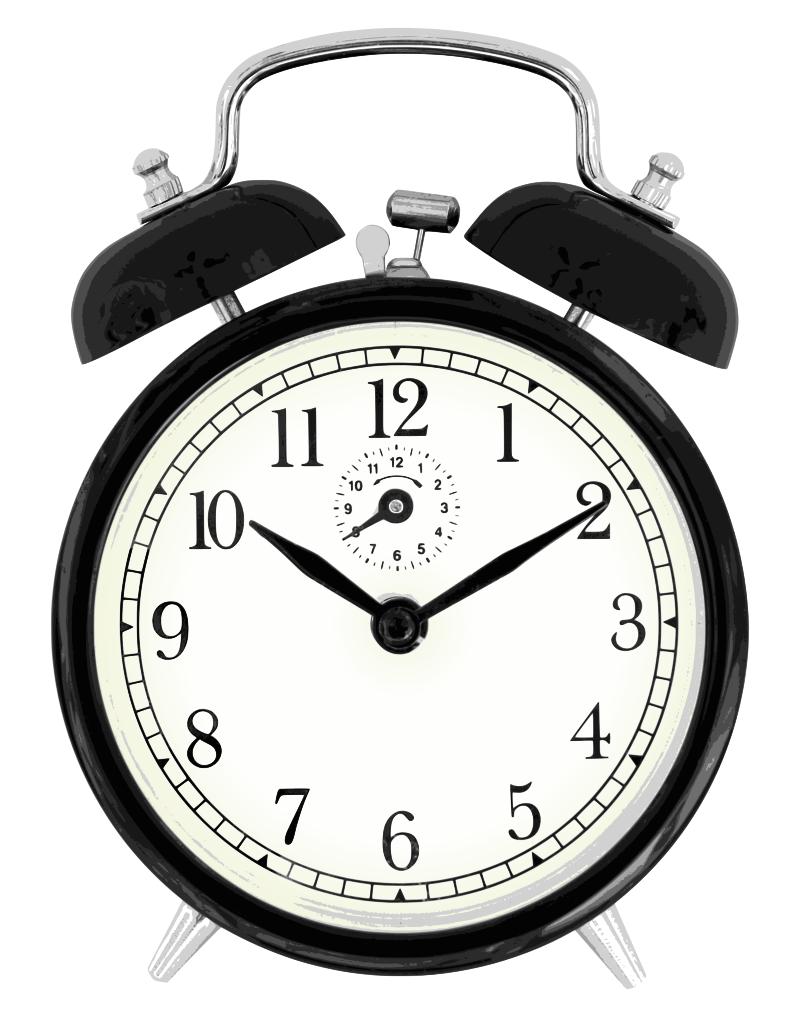
\includegraphics[width=6cm]{img/clock.png}}

%Make the Header
\makeatletter
\let\runauthor\@author
\let\runtitle\@title
\makeatother
\rhead{\runauthor}
\chead{\runtitle}
\lhead{\begin{picture}(0,0) \put(0,0){
\includegraphics[scale=0.5]{img/bfh.png}} \end{picture}}



\begin{document}

\thispagestyle{empty}
\maketitle
\tableofcontents

\pagestyle{fancy}


\begin{abstract}
\end{abstract}
%\section{Zweck des Dokument}
\chapter{Zweck des Dokument}
Dieses Dokument soll dazu dienen, die Anforderungen an das Projekt AlarmClock zu definieren. Typische Leser sind die
Entwickler und der Dozent im Requirements Engineering. Auch für den Projektbetreuer kann das Dokument von Interesse sein.
%makes sure the whole glossary gets printed even when acronyms are not defined

\section{Kurzbeschreibung}
Das Ziel des Projektes ist einen Ersatz zum Programm kAlarm zu entwickeln.
Das Programm kAlarm erlaubt es dem User benutzerdefinierte Erinnerungen zu erstellen. Mittels Pop-Up Windows wird der
User dann zur gegebenen Zeit daran erinnert. Im Gegensatz zu kAlarm soll das zu erstellende Produkt
platformübergreifend verfügbar sein. Wie kAlarm soll dieses Produkt unter einer Open Source Lizenz entwickelt werden.

\section{Projektziele}
Unser Auftraggeber ist kein Unternehmen. Es werden somit auch keine Ziele innerhalb eines Unternehmens verfolgt.
Ziele, welche ein Benutzer unsere Aplikation verfolgen könnte wären beispielsweise:
\begin{itemize}
 \item An den Wäschetag erinnert weden.
 \item Die Wäsche rechtzeitig aus der Wäscheküche holen.
 \item Den Kuchen nicht im Backofen verbrennen lassen.
 \item Der Sekretärin zum Geburtstag Blumen schicken.
 \item usw.

\end{itemize}

\section{Stakeholders}
\begin{itemize}
\item{Auftragsgeber: Prof. Claude Furrer}
\item{Auftragsnehmer: Jonathan Hyams, Pascal Schmalz}
\item{Benutzer: FOSS Communitiy}
\end{itemize}
\section {Systemabgrenzung}
Es exisitert kein vordefiniertes System, welches mit unserem Programm interagiert.
Das Programm soll auf einem Computer laufen, welcher Java 8.1 inklusive JavaFx installiert hat.
 
\subsection{Geschäftsprozesse}
Es existieren keine vor\- oder nachgelagerte Prozesse. Unsere Lösung lässt sich in beliebig viele Prozesse integrieren.
\subsection{Systeme}
Unser System beinhaltet einen Persistenz Layer um nach einem Neustart den vorherigen Zustand wiederherstellen zu können.
Die Persistenz soll an einem zentralen Punkt sichergestellt werden, so dass mit wenig Aufwand eine andere
Persistenzmethode, wie eine JPA Datenbank eingebunden werden kann.

\begin{landscape}
\begin{figure}
  \centering
    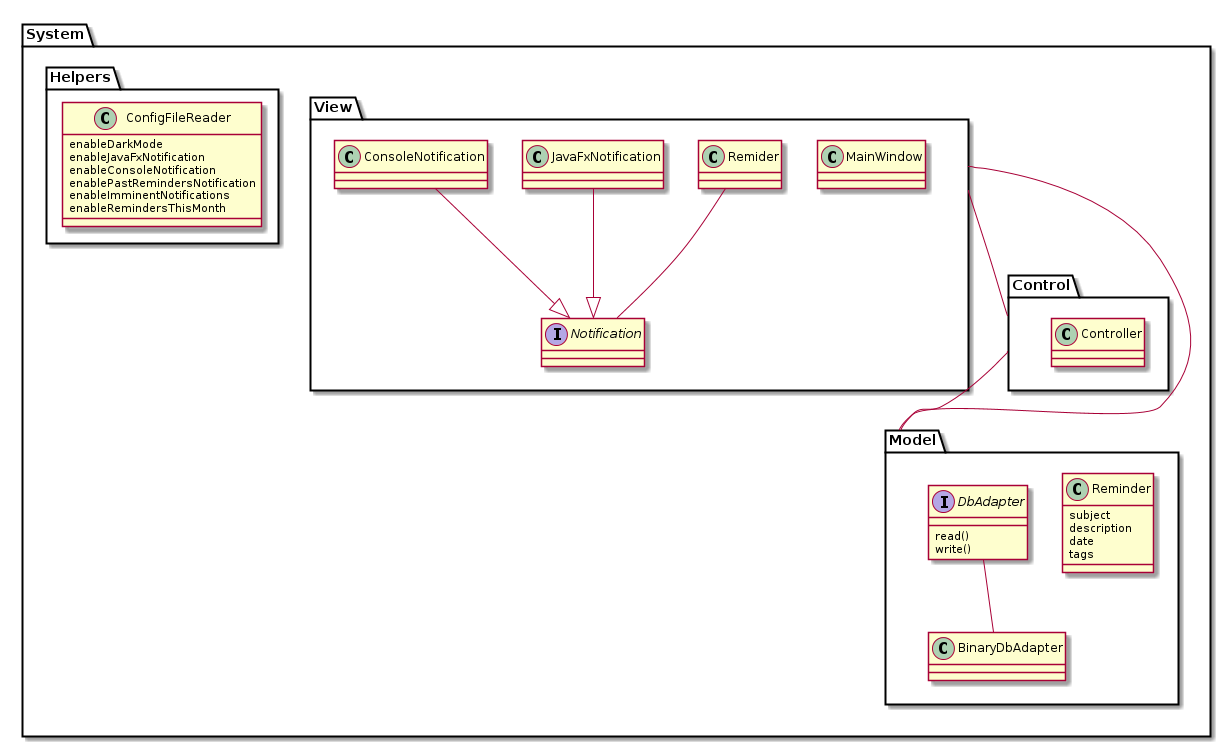
\includegraphics[width=1\textwidth]{../uml/uebersicht.png}
  \caption{Systemübersicht und Abgrenzung}
  \label{fig:overview}
\end{figure}
\end{landscape}
Die Systemübersicht und Abgrenzung Abb.~\ref{fig:overview} Seite~\pageref{fig:overview} bedient sich der UML Notation,
ohne die UML Spezifikation vollständig einzuhalten. Die Komponenten innerhalb des Kasten ``System'', insbesondere ihre
Beziehung zueinander, sind nicht Teil der Anforderungen, und somit nicht bindend. Sie veranschaulichen lediglich was
noch innerhalb des Systems liegt und was ausserhalb
angesiedelt ist.
Abbildung:\pageref{fig:overview}




Falls die Funktionalität vom Auftraggeber verlangt wird, muss das Programm den Nutzer mit E-Mails, SMS und
Systemnotifications erinnern. Dies bedingt, dass entsprechende Services / Server eingerichtet und über eine definierte
Schnittstelle erreichbar sind, was nicht mehr Teil des Projektes ist.

\subsection{Randbedingungen}
Die Entwicklung soll mittels Java und JavaFX erfolgen.
Das Programm soll Betriebssystem und Datenbank agnostisch sein. Das Projekt muss unter einer Opensource Lizenz
veröffentlicht werden.
Die Dokumentation muss in \LaTeX ~erstellt werden.


\section{Anforderungen}
\subsection{Basisfaktoren}
\begin{itemize}

\item Die Schnittstelle zwischen dem Programmcode und der Datenbank soll so gestaltet sein, dass mit einem minimalen
Aufwand eine beliebige gängige Datenabank genutzt werden kann.


\item
Die Bereitstellung eines JPA Drivers der Datenbank ist dabei nicht mehr im Scope des Projektes, sondern wird von den
Datenbankherstellern oder von Dritten vorgenommen.

\item
Das System muss dem Benutzer die Möglichkeit bieten, in dem GUI ein Einzelevent zu erfassen.


\item
Das System kann anderen Programmen über eine API ermöglichen, Einzelevents zu erfassen.

\item
Das Löschen von Events soll wie oben beschrieben, ebenfalls möglich sein.


\item
Das System muss den Benutzer mittels einer Notification vorzeitig, am Tag des  Events Zeit, auf ein Event hinweisen.
\item
Das System muss den Benutzer mittels einer Notification rechtzeitig, zur voreingestellten Zeit, auf ein Event hinweisen.

\item
Das Programm muss an einem Zentralen Ort konfiguriert werden.

\end{itemize}

\subsection{Leistungsfaktoren}
\begin{itemize}
\item
Der Benutzer soll neue Kategorien hinzufügen, anpassen und löschen können.
\item
Events sollen durch den Benutzer in Kategorien eingeteilt werden können.
\item
Der Benutzer soll Events nach Kategorien gruppieren und filtern können.
\item
Das Programm soll vorkonfigurierte Dienste nutzen können um seine Notifications als SMS und Emails zu versenden.
\item
Das Programm soll vorkonfigurierte Dienste nutzen können um anstelle einer Notification ein Script laufen zu lassen.
\item
Die GUI soll Benutzerzentriert und Ergonomisch sein.
\end{itemize}

\subsection{Begeisterungsfaktoren}


\begin{itemize}
\item
Das Programm soll vorkonfigurierte Dienste nutzen können um anstelle einer Notification  ein IFTTT Event auszulösen.

\item
Das Programm soll zusätzlich zu den gängigen Computer-Betriebssystemen auch auf Android lauffähig sein.


\item
Das Programm soll auf den Betriebssystemen, welche eine Notificationinfrastruktur bereitstellen  in der Lage sein die Notifications über diese vorzunehmen.(BSP KDE)

\item
Das Programm soll sich vom Look and Feel in die jeweilige Desktop Environment anpassen.
\item
Das System kann dem Benutzer die Möglichkeit bieten, in dem GUI wiederkehrende Events zu erfassen.
\item
Das Programm kann dem Benutzer die Möglichkeit bieten, die Konfiguration über die GUI vorzunehmen und im Configfile zu speichern.

\end{itemize}






 %IFTTT
\subsection{Quellen und Vorgehen}
Unsere wichtigste Quelle ist unser Auftraggeber Prof. Furrer. Um die Fragen, welche bei der Erstellung der
Anforderungen aufgetaucht sind zu klären, werden wir uns mit ihm treffen. Besondere folgende Fragen gilt es abzuklären:

\begin{itemize}
\item Entspricht die bisherige Ausarbeitung der Vorstellung des Auftraggebers.
\item Vollständigkeit der Anforderungen.
\item Kategoriserung der Anforderungen.
\item Priorisierung der Anforderungen.
\item Was soll mit der Eventkategorisierung erreicht werden, welche weiteren Anforderungen ergeben sich daraus.
\item Abgrenzung des Programmes gegenüber eines kAlarm, Kalenders und gegenüber des Cronjobs.
\end{itemize}
Da unser Auftraggeber als Professor der Informatik tätig ist, ist das Glossar für unseren Auftraggeber obsoloet. Der Vollständigkeihthalber wird es dennoch erstellt. 
Als weitere Diskusionsgrundlage sind wir daran neben diesem Dokument einen Prototyp des GUI zu erstellen.
Da wir selber der potentiellen Nutzergruppe des Programmes angehören, könnten wir auch uns selber als Quelle nutzen, als Entwickler hat man jedoch oft einen anderen Blickwinkel als ein normaler Benutzer.
Auch das Feedback von Komilitonen war uns ein anhaltspunkt.
Im Sinne einer agilen Entwicklung wollen wir möglichst rasch präsentierbare Artefakte generieren, damit der Auftraggeber frühstmöglich Einfluss nehmen kann und Fehlentwicklungen vermieden werden. Treffen werden bei Bedarf mit dem Auftraggeber ausgemacht.


\subsection{Technische Anforderungen}

\begin{itemize}
 \item Das Programm muss auf Linux, Windows und OSx lauffähig sein.
 \item Das Programm muss datenbankagnostisch sein.
 \item Das Programm muss auf dem Buildsystem kompiliert werden können.
 \item Das Programm muss auf dem Referenzsystem ohne weitere installationen kompiliert werden können.
\end{itemize}



\subsection{Qualitätsanforderungen}
\begin{itemize}
\item 80\% der Benutzer sollen in der Lage sein, ohne vorgänige Schulung, bei der ersten Benutzung, folgende Aktionen
jeweils innert 5 Minuten nach erfolgtem Programmstart, auszuführen:
\begin{itemize}
\item Erstellen eines Events.
\item Löschen eines vorhandenen Events.
\item Editieren eines Events (Zeit, Datum, Notificationtext).
\end{itemize}

\item 60\% der Benutzer solle in der Lage sein, die Konfiguration des Programmes mittels ConfigFiles Vorzunhemen.
\end{itemize}makeglossaries document

\section{Anhang}
\listoffigures
\listoftables
\glsaddall
\printglossary
%TODO bibography

\glsaddall
\printglossary
\subsection{Qualitätsaspekt Inhalt}
Folgende Punke sind vorhanden:
\begin{itemize}
 \item Vollständigkeit als Menge aller Anforderungen.
 \item Vollständig der einzelnen Anforderungen.
 \item Korrektheit der Anforderungen.
 \item Konsistezn
 \item Keine vorzeitigen Entwurfscentscheidungen.
 \item Die Überprüfbarkeit ist gegeben. Es werden jedoch nicht alle Anforderungen einzeln überprüft. Als Erfolgskriterien dienen verkürzten Userstotys mit genau angegebenen Metriken zur Überprüfbarkeit.
 \item Notwendigkeit
\end{itemize}
\subsection{Qualitätsaspekt Dokumentation}
Da wir nur einen Steakholder haben, ist es gegeben ,dass auch die relevanten Stakholder zugange sind. Laut Lehrbuch sollte es vermieden werden, dass die Anforderungen von den Erstellern überprüft werden. Da unser Betreuer sich aber verständlicherweise primär für die Artefakte des eigentlichen Entwicklungsprozesses interessierte, haben wir als Ersteller diese Dokumentation systematisch geprüft. Externe Überprüfer sind nicht angezeigt, da die Anforderungen keinem genügend hohen Qualitätsgrad genügen müssen.

Das Prinzip der Trennunb von Fhelersuche und Fehlerkorrektur haben wir nicht strikt eingehlten. Da die Fehlersucher und die Korrekture onehin dieselben Personen sind, war dies schwierig. Gerade bei kleinen Fehlern ist das korrigieren dieser rasch erledigt. Eine zusätzliche Dokumentation als Zwischenschritt hätte einen Mehraufwand bedeutet die angedeutete Gefahr beim Zusammenlegen der Schritte hielten wir in diesem Rahmen als überschaubar.

Die überprüfung aus unterschiedlichen Sichten konnten wir zu zweit durchspielen, indem eine Person aus der Sicht eines potentiellen Users argumentierte.
Für den grossteil dieser Dokumentation haben wir uns auf Texte als Dokumentationsform beschränkt. Lediglich die Abbildung ~\ref{fig:overview} auf Seite~\pageref{fig:overview} haben wir schematisch dargestellt.

Entwicklungsartefakte als teil es Anforderungsanalyse spielen vorallem in der Agilen Entwicklung eine wichtige Rolle. Diese werden dort aber vorallem als teil der Entwicklung  betrachtet. Dementsprechend haben wir hier auch keine solchen beigelgt, sondern verweisen auf unse Github Code Repository, welches wir gerne für Sie freischalten, wenn Sie uns ihren Github Username angeben.


\subsection{Qualitätsaspekt Abgestimmtheit der Anforderungen}
Die Abstimmun der Anforderungen 
Unser Betreuer wollte uns im sinne einer Agilen Entwicklung eine grösstmögliche Freiheit lassen.Änderungswünsche an diesem Dokument wurden von ihm keine angebracht. Da es sich um keine Auftragsarbeit für ein komerzielles Unternehmen handelt, bildet dieses Dokument auch keine Vertragsgrundlage.

Obwohl wir Unterschiedliche Steakholder aufgelistet haben, gibt es in diesem Projekt einen klaren Entschiedungsträger, unser Betreuer. Prof. Furrer. Die Open Source Gemeinde selber ist so heterogen und verstreut, dass  eine Abstimmung der Wünsche mit der gesamten Comunity onehin zum scheitern verurteilt wäre.

Ohne Zielkonflikte hatten wir auch keine Gelegenheit diese als Chance zu nutzen um neue Ideen zu entwickeln. Der Start der Entwicklungsphase dürfte laut dem Requirements Engineering Prozess erst erfolgen, nachdem die Abstimmung der Anforderungen erfolgt ist.
Durch die Struktur des Unterrichts war es aber so gegeben, dass der Start der Entwicklungsphase  mit dem Start der Anforderungsanalyse zusammen fielen.Für eine rein agile Vorgehensweise ist dies kein Problem. Will man das Requirements Engineering jedoch wie gefordert vor der Entwicklungsphase abschliessen, müsste man die Entwicklungsphase in einem späteren Semester starten.



Hier offenbart sich wohl ein Unterschied zwischen  einem agilen Entwicklungsprozess und dem System Engineering.
\subsection{Definition of Ready - Checklist}
Wie bereits erwähnt, passt unser Projekt nicht optimal zur Vorgehensweise, welche wir im Requirements Engineering betrachtet haben. Wir haben mit unserem Betreuer auch keine vollumfängliche Definitino of Ready für die Anforderung ausgearbeitet. Die drei oben erwähnten Qualitätsaspekte haben wir wie beschrieben abgehandelt. 
\section{Versionskontrolle}
Manuelle Version: 0.1.0
\\

\noindent
Automatische Versionierung:
\immediate\write18{../script/versionInfo.sh}
Fetching version information failed. Please enable shell-escape in your \LaTeX \~  compiler.

\immediate\write18{../script/cleanup.sh}
%\immediate\write18{../script/clean.sh}







\end{document}
